The goal of this section is to prove that ReLU nets can approximate continuous functions $f: K \to \bb{R}$, where $K$ is compact (for a formal statement see Theorem \ref{infinitecase} below). This will be done by approximating a continuous function $f: \bb{R}^2 \to \bb{R}$ on a compact subset $K \subseteq \bb{R}^2$. Again, a ReLU net which approximates $f$ itself will not be directly constructed, but a max-min string will be instead, which is sufficient by Lemma \ref{maxmin}.\\\\
%
In the finite case, a max-min string $g: S\setminus\lbrace s \rbrace \to \bb{R}^m$ was extended to $\hat{g}: S \to \bb{R}^m$. The existence of $\hat{g}$ used crucially that there existed an affine function $l: \bb{R}^n \to \bb{R}^m$ such that each entry of $l(s')$ was larger than the corresponding entry of $g(s')$, for all $s' \in S\setminus\lbrace s \rbrace$, and was such that $l(s) = 0$. The key realisation in the case where $K$ is an arbitrary compact set is the existence of an analogous affine function $l$:
%
\begin{defn}
The \textbf{inverse modulus of continuity of $\epsilon$} of a continuous function $f: \bb{R}^2 \to \bb{R}$ in the domain $K \subseteq \bb{R}^2$ is
\[w_{f,K}^{-1}(\epsilon) = \operatorname{sup}\lbrace \delta \in \bb{R} \mid \forall x, y \in K\text{, }|x - y| \leq \delta \Rightarrow |f(x) - f(y)| \leq \epsilon\rbrace\]
\end{defn}
%
%
%
%
%
%
%
%
%
%
\begin{lemma}
\label{circlelemma}
Let $f: \bb{R}^2 \to \bb{R}$ be continuous, $\epsilon > 0$, $r > r' > 0$. Let $S_r := \lbrace (x,y) \in \bb{R}^2 \mid x^2 + y^2 = r \rbrace$ be the circle of radius $r$. Let $X,Y \in S_r$ be such that $|X - Y| \leq r$ and $X',Y' \in S_{r'}$ be such that $X',X,Y,Y'$ are collinear, and let $Z \in S_{r'}$ be the point on the arc connecting $X'$ to $Y'$ and the straight line which passes through the origin and the midpoint of the straight line connecting $X$ and $Y$. See Figure \ref{elelprime}.
\begin{figure}[h]
    \centering
    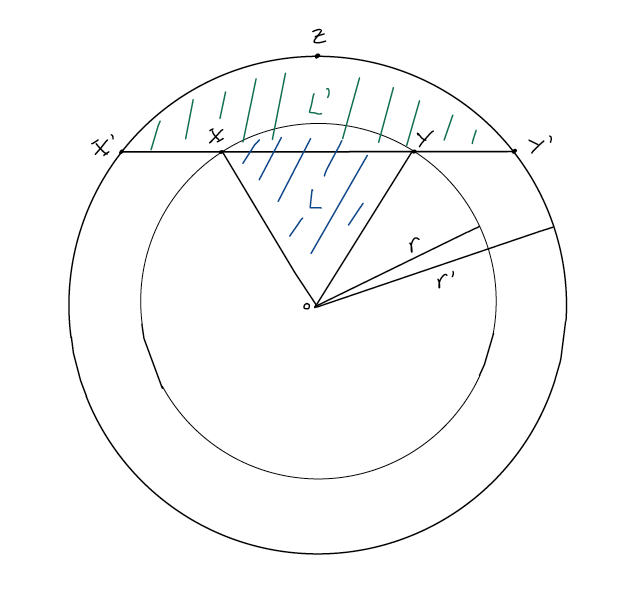
\includegraphics[width=20em]{Sections/Diagrams/elelprime.png}
    \caption{The configuration described in Lemma \ref{circlelemma}}
    \label{elelprime}
\end{figure}
Let $L$ denote the minor sector of $S_r$ induced by the radii $0X$ and $0Y$ and let $L'$ denote the minor segment of $S_{r'}$ induced by the chord which connects $X'$ to $Y'$. If
\[\operatorname{Diam}(L') \leq w_{f,B_{r'}(0)}^{-1}(\epsilon)\]
then there exists an affine function $l: \bb{R}^2 \to \bb{R}$ such that
\begin{itemize}
    \item $l(x) \leq \epsilon$ for all $x \in L'$,
    \item $|f(x) - f(Z)| \leq l(x) + \epsilon$ for all $x \in L$.
\end{itemize}
\end{lemma}
%
%
%
%
%
%
%
%
%
%
%
\begin{proof}
Let $l$ be the affine function such that $l(Z) = 0$ and $l(X') = l(Y') = \epsilon$. Let $x \in L$. Denote by $Z' \in \bb{R}^2$ the point which is collinear to $X',Y',X,Y$ and is also collinear to $Z,x$. Then as $l$ is affine and $|x - Z| \leq |Z' - Z|$, it follows that $l(x) \leq l(Z') = \epsilon$.\\\\
%
Say $x \in L'$. Then write $|x - Z| = kw_{f,B_{r'}(0)}^{-1}(\epsilon) + \rho$ where $k \in \bb{N}$ and $0 \leq \rho < w_{f,B_{r'}(0)}^{-1}(\epsilon)$. Then
\begin{align*}
    &|x - Z| = kw_{f,B_{r'}(0)}^{-1}(\epsilon) + \rho\\
    &\Rightarrow |x - Z| \geq kw_{f,B_{r'}(0)}^{-1}(\epsilon)\\
\end{align*}
and so,
\begin{equation}
\label{integerandremainder}
    \frac{\epsilon |Z - x|}{w_{f,B_{r'}(0)}^{-1}(\epsilon)} \geq k\epsilon
\end{equation}
Also, consider a sequence of points $Z = x_1,x_2,...,x_{k+1} = x$ such that $|x_{i+1} - x_i| = w_{f,B_{r'}(0)}^{-1}(\epsilon)$ for $i = 1,...,k-1$ and $|x_{k+1} - x_k| < w_{f,B_{r'}(0)}^{-1}(\epsilon)$. See Figure \ref{devastation}.
\begin{figure}
    \centering
    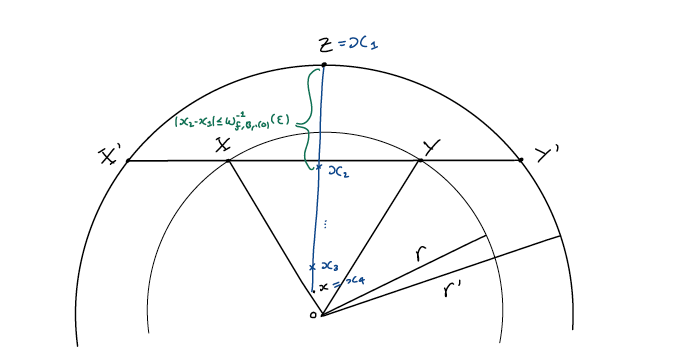
\includegraphics[width = 40em]{Sections/Diagrams/devastation.png}
    \caption{The points $x_1,...,x_n$ in the proof of Lemma \ref{circlelemma}}
    \label{devastation}
\end{figure}Then
\begin{align*}
    |f(x) - f(Z)| &= |f(x_1) - f(x_2) + f(x_2) - f(x_3) + ... + f(x_2) - f(x_1)|\\
    &\leq |f(x_1) - f(x_2)| + ... + |f(x_2) - f(x_1)|\\
    &< k\epsilon + \epsilon
\end{align*}
and so,
\begin{equation}
    \label{triangleineq}
    |f(x) - f(Z)| < k\epsilon + \epsilon
\end{equation}
Equations \ref{integerandremainder} and \ref{triangleineq} together imply
\[|f(x) - f(Z)| < \frac{\epsilon |x - Z|}{w_{f,B_{r'}(0)}^{-1}(\epsilon)} + \epsilon\]
Thus it remains to show:
\[\frac{\epsilon |x - Z|}{w_{f,B_{r'}(0)}^{-1}(\epsilon)} \leq l(x)\]
This comes down to the fact that the slope of $l$ in the direction of the vector $x - Z$ can be bounded below by $\frac{\epsilon}{w_{f,B_{r'}(0)}^{-1}(\epsilon)}$. More precisely, consider the following parametrisation of the straight line which intersects $Z$ and $x$:
\begin{align*}
    c: \bb{R} &\to \bb{R}^2\\
    s &\mapsto Z + \frac{s}{|x - Z|}(x - Z)
\end{align*}
Then the function $lc: \bb{R} \to \bb{R}$ is affine, and in fact is linear as
\[lc(0) = l(Z) = 0\]
So for all $y \in \bb{R}$, $lc(y) = my$ for some gradient $m$. Let $W \in \bb{R}^2$ be the point which intersects the line parametrised by $c$ and the line which passes through $X$ and $Y$. Then since $|W - Z| \leq w_{f,B_{r'}(0)}^{-1}(\epsilon)$ and $l(W) = \epsilon$, it follows that:
\[m = \frac{l(W) - l(Z)}{|W - Z|} = \frac{\epsilon}{|W - Z|} \geq \frac{\epsilon}{w_{f,B_{r'}(0)}^{-1}(\epsilon)}\]
and so:
\[\frac{\epsilon |x - Z|}{w_{f,B_{r'}(0)}^{-1}(\epsilon)} \leq m|x - Z| = lc(|x - Z|) = l(x)\]
which completes the proof.
\end{proof}
%
%
%
%
%
%
%
%
%
%
%
\begin{cor}
\label{cor:geometric-maxmin}
In the setting of Lemma \ref{circlelemma}, but with every instance of $\epsilon$ replaced by $\frac{\epsilon}{2}$, if there exists a max-min string $g: \bb{R}^2 \to \bb{R}$ which approximates $f$ on $L'$ then there exists a max-min string $\hat{g}: \bb{R}^2 \to \bb{R}$ which approximates $f$ on $L \cup L'$.
\end{cor}
%
%
%
%
%
%
%
%
%
%
%
\begin{proof}
Let $l: \bb{R}^2 \to \bb{R}$ be an affine function such that
\begin{itemize}
    \item $l(x) \leq \frac{\epsilon}{2}$, for all $x \in L'$,
    \item $|f(x) - f(Z)| \leq l(x) + \frac{\epsilon}{2}$, for all $x \in L$
\end{itemize}
the existence of which is guaranteed by Lemma \ref{ballapprox}. Then define the max-min string
\[\hat{g} = \operatorname{max}\lbrace \operatorname{min}\lbrace g, f(Z) + l\rbrace, f(Z) - l\rbrace\]
On $L$, we have $f \leq g + \epsilon$ and
\[f\leq f(Z) + l + \epsilon\]
so
\begin{align*}
    f &\leq \operatorname{min}\lbrace g + \epsilon, f(Z) + l + \epsilon\rbrace\\
    &= \operatorname{min}\lbrace g, f(Z) + l\rbrace + \epsilon\\
    &\leq \operatorname{max}\big\lbrace\operatorname{min}\lbrace g, f(Z) + l \rbrace, f(Z) - l\big\rbrace + \epsilon\\
    &= \hat{g} + \epsilon
\end{align*}
Similarly, since $g - \epsilon \leq f$ and
\[f(Z) - l - \epsilon \leq f\]
it follows that
\begin{align*}
    \hat{g} - \epsilon &= \operatorname{max}\big\lbrace \operatorname{min}\lbrace g, f(Z) + l - \epsilon\rbrace, f(Z) - l\big\rbrace - \epsilon\\
    &= \operatorname{max}\lbrace \operatorname{min}\lbrace g - \epsilon, f(Z) + l - \epsilon\rbrace, f(Z) - l - \epsilon\rbrace\\
    &\leq \operatorname{max}\lbrace g - \epsilon, f(Z) - l - \epsilon\rbrace\\
    &\leq f
\end{align*}
On $L'$, by construction:
\[f(Z) - \frac{\epsilon}{2} \leq f(Z) - l \leq \hat{g} \leq f(Z) + l \leq f(Z) + \frac{\epsilon}{2}\]
and for all $x \in L'$
\[|f(x) - f(Z)| \leq \frac{\epsilon}{2}\]
by definition of $w_{f,B_{r'}(0)}^{-1}(\frac{\epsilon}{2})$. Thus:
\begin{align*}
    |\hat{g}(x) - f(x)| &= |\hat{g}(x) - f(Z) + f(Z) - f(x)|\\
    &\leq |\hat{g}(x) - f(Z)| + |f(Z) - f(x)|\\
    &\leq \frac{\epsilon}{2} + \frac{\epsilon}{2}\\
    &= \epsilon
\end{align*}
%
\end{proof}
%
%
%
%
%
%
%
%
%
%
%
Next we turn to two geometric Lemmas:%
%
%
%
%
%
%
%
%
%
%
%
\begin{lemma}
\label{elementarygeometryone}
Consider two concentric circles, $S_R$ and $S_{R'}$ with $R' > R$. Consider a chord intersecting points $X$ and $Y$ on $S_R$ and extend this chord so that it intercepts $S_{R'}$, at $X'$ and $Y'$ say (see Figure \ref{fig:elementarygeometryone}). Then
\[|X'Y'|^2 = 4(R'^2 - R^2) + |XY|^2\]
\end{lemma}
\begin{proof}
Let $P$ denote the midpoint of the line $XY$. Then $|P| = \sqrt{R^2 - \frac{1}{4}|XY|^2}$ (again, see Figure \ref{fig:elementarygeometryone}).
\begin{figure}
    \centering
    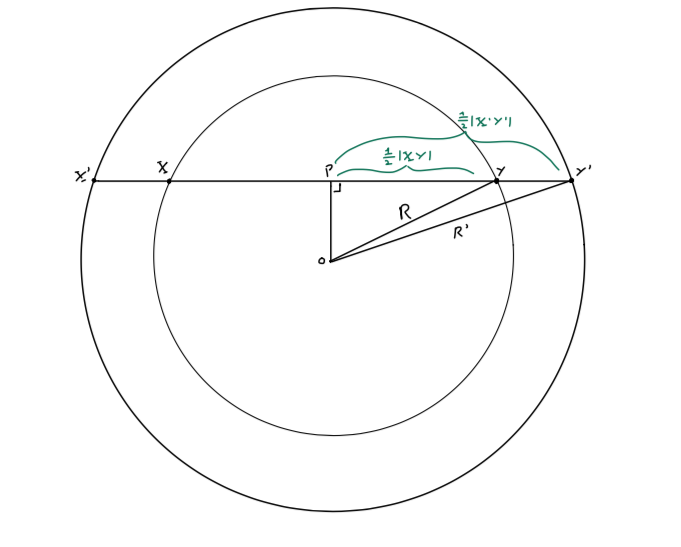
\includegraphics[width = 25em]{Sections/Diagrams/elementarygeometry.png}
    \caption{The geometry of Lemma \ref{elementarygeometryone}}
    \label{fig:elementarygeometryone}
\end{figure}
Thus
\begin{equation*}
    \Big(\sqrt{R^2 - \frac{1}{4}|XY|^2}\Big)^2 + \frac{1}{4}|X'Y'|^2 = R'^2
\end{equation*}
from which, the result follows.
\end{proof}
%
%
%
%
%
%
%
%
%
%
\begin{lemma}
\label{elementarygeometrytwo}
Let $X,Y$ be points on $S_R$ such that $0 < |X - Y| \leq R$. Let $\tau_X$ and $\tau_Y$ be straight lines tangent to $S_R$ respectively at $X$ and $Y$. Let $T$ denote the intersection of $\tau_X$ and $\tau_Y$. Then $\operatorname{Diam}(\Delta XTY) = |X - Y|$
\end{lemma}
%
%
%
%
%
%
%
%
%
%
\begin{proof}
If $|X - Y| = R$ then the triangle $XOY$ is equilateral. It follows from this that angle $\angle TXY$ and $\angle TYX$ are both equal to $30^\circ$. As $|X - Y|$ decreases, both angles $\angle TXY$ and $\angle TYX$ decrease. So if $|X - Y| \leq R$ the angle $\angle XTY$ is obtuse, which implies that $\operatorname{Diam}(\Delta XTY) = |X - Y|$. See Figure \ref{fig:elementarygeometrytwo}.
\begin{figure}
    \centering
    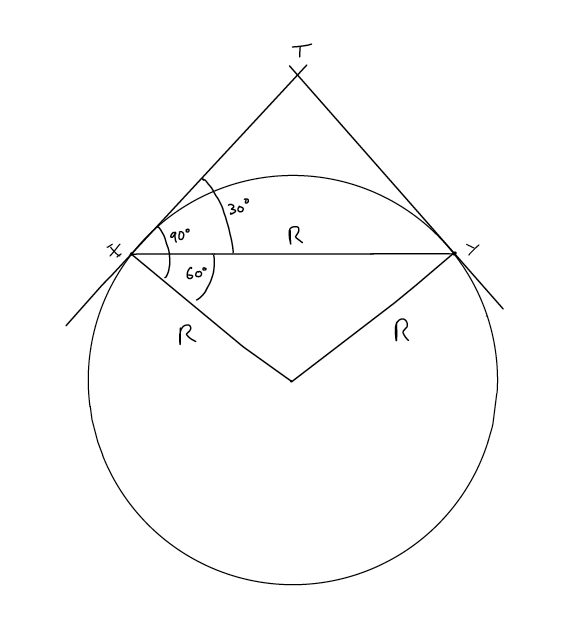
\includegraphics[width = 20em]{Sections/Diagrams/elementarygeomtwo.png}
    \caption{The geometry of Lemma \ref{elementarygeometrytwo}}
    \label{fig:elementarygeometrytwo}
\end{figure}
\end{proof}
%
%
%
%
%
%
%
%
%
%
%
\begin{lemma}
\label{ballapprox}
Let $f: \bb{R}^2 \to \bb{R}$ be continuous, $\epsilon > 0$, $R > 0$. Assume $w_{f,B_{R}(0)}^{-1}(\frac{\epsilon}{2})$ and let $R' > w_{f,B_{R}(0)}^{-1}(\frac{\epsilon}{2})$. Assume further that there exists a max-min string $g: \bb{R}^2 \to \bb{R}$ which approximates $f$ on $B_{R'}(0)$. Let $R''$ be
\[R'' := \sqrt{R'^2 + \frac{w_{f,B_{R}(0)}^{-1}(\frac{\epsilon}{2})}{\sqrt{2}R'}}\] If $R'' < R$ then there exists a max-min string $\hat{g}: \bb{R}^2 \to \bb{R}$ which approximates $f$ on $B_{R''}(0)$, and if $R'' \geq R$ then there exists a max-min string $\hat{g}: \bb{R}^2 \to \bb{R}$ which approximates $f$ on $B_{R}(0)$.
\end{lemma}
%
%
%
%
%
%
%
%
%
%
\begin{proof}
To ease notation let $a_{R'} := \frac{w_{f,B_{R}(0)}^{-1}(\frac{\epsilon}{2})}{\sqrt{2}R'}$. Let $X,Y \in \bb{R}^2$ lie on the circle of radius $R'$ which satisfy
\[|XY| = w_{f,B_{R}(0)}^{-1}(\frac{\epsilon}{2})(1 - a_{R'})^{\frac{1}{2}}\]
such a pair $(X,Y)$ exists as
\[|XY|^2 = w_{f,B_{R}(0)}^{-1}(\frac{\epsilon}{2})^2(1 - a_{R'}^2) < w_{f,B_{R}(0)}^{-1}(\frac{\epsilon}{2}) \leq R'\]
We consider first the case when $R'' < R$. Let $X',Y' \in \bb{R}^2$ lie on the circle of radius $R''$ which intersect the line segment connecting $X$ and $Y$. Let $L$ denote the minor segment on the circle of radius $R'$ induced by the chord which connects $X'$ to $Y'$ and let $L'$ denote the minor sector on the circle of radius $R'$ induced by the radii $0X$ and $0Y$. Let $Z$ denote the intersection of the circle of radius $R''$ and the line which connects $0$ and the midpoint of the line $XY$. See Figure \ref{ballconfig}.
\begin{figure}
    \centering
    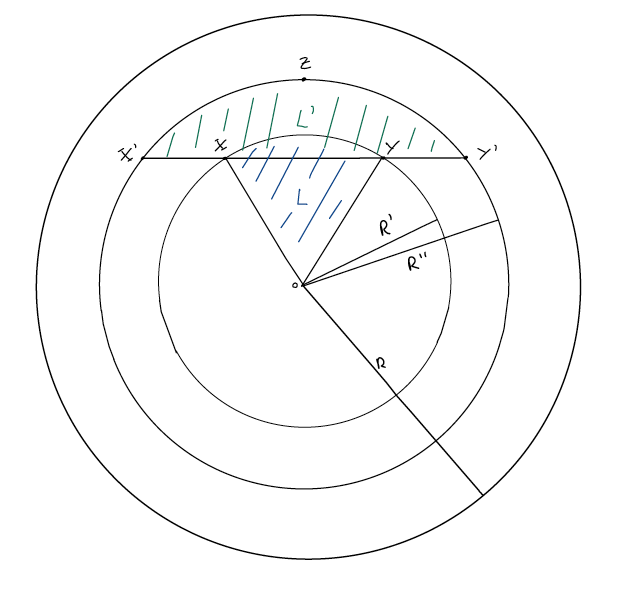
\includegraphics[width=20em]{Sections/Diagrams/ballconfig.png}
    \caption{Configuration of the balls in Lemma \ref{ballapprox}}
    \label{ballconfig}
\end{figure}
By Lemma \ref{elementarygeometryone} and a direct calculation,
\[|X'Y'| = \sqrt{4(R^{''2} - R^{'2}) + |XY|^2} = w_{f,B_{R}(0)}^{-1}(\frac{\epsilon}{2})\]
Moreover, $w_{f,B_{R}(0)}^{-1}(\frac{\epsilon}{2}) < R' < R''$, so by Lemma \ref{elementarygeometrytwo}:
\[\operatorname{Diam}(L) \leq w_{f,B_{R}(0)}^{-1}(\frac{\epsilon}{2})\]
Thus the hypotheses of Corollary \ref{cor:geometric-maxmin} are satisfied.\\\\
%
The case when $R'' \geq R$ is almost identical but the pair $(X',Y')$ are taken to intersect the ball of radius $R$ instead of the ball of radius $R''$.
\end{proof}
%
%
%
%
%
%
%
%
%
%
%
This brings us to the main Theorem:
\begin{thm}
\label{infinitecase}
Let $\epsilon \in \bb{R}_{>0}$ and $f: \bb{R}^2 \to \bb{R}$ be continuous, and $K \subseteq \bb{R}^2$ compact. Then there exists a max-min string $g: \bb{R}^2 \to \bb{R}$ such that
\[\forall x \in K,\text{ }|g(x) - f(x)| \leq \epsilon\]
\end{thm}
\begin{proof}
Since compact subsets of $\bb{R}^2$ are bounded, it suffices to consider the case when $K = B_R := \lbrace x \in \bb{R}^2 \mid |x| \leq R\rbrace$, for some $R \in \bb{R}$. If $R \leq w_{f,B_{R}(0)}^{-1}\big(\frac{\epsilon}{2}\big)$ then the max-min string $g: \bb{R}^2 \to \bb{R}$ which is the constant function $g \equiv f(0)$ suffices. Suppose $w_{f,B_{R}(0)}^{-1}\big(\frac{\epsilon}{2}\big) < R$ and $f: B_R(0) \to \bb{R}$ are given. Consider the following set
\[\scr{X} := \lbrace R' \in \bb{R} \mid \text{there exists a max-min string } g\text{ which approximates }f\text{ on }B_{R}(0)\rbrace\]
We claim that $R \in \scr{X}$, recall the notation from Lemma \ref{ballapprox} that $a_R := \frac{w_f^{-1}\big(\frac{\epsilon}{2}\big)^2}{\sqrt{2}R}$. Suppose for a contradiction that $R \not\in \scr{X}$, then $\scr{X}$ is bounded above. Let $s^2 = \sup\scr{X}^2$ and $R' \in \scr{X}$ to be such that
\[s^2 - a_s < R'^2\]
Notice that $s \not\in \scr{X}$ as if $s \in \scr{X}$ then Lemma \ref{ballapprox} can be used to find a strictly greater value in $\scr{X}$. As $R' < s$, it follows that $a_s < a_{R'}$ and
\[s^2 < R'^2 + a_s < R'^2 + a_{R'}\]
thus
\[s < \sqrt{R'^2 + a_{R'}}\]
but by Lemma \ref{ballapprox}, $\sqrt{R'^2 + a_{R'}} \in \scr{X}$, contradicting that $s$ is a supremum.
\end{proof}

\begin{remark}
\label{bound}
As mentioned earlier, Theorem \ref{infinitecase} generalises to continuous functions $f: K \to \bb{R}^m$ where $K \subseteq \bb{R}^n$. Ie, given $\epsilon > 0$ there exists a max-min string $g: \bb{R}^n \to \bb{R}^m$ such that for all $x \in K$,
\[|f(x) - g(x)| < \epsilon\]
Lemma \ref{maxmin} then implies that there exists a ReLU net with input width $n$ and all other widths equal to $n + m$ which approximates $f$. This gives the promised upper bound on the widths. In fact a lower bound can be proved as well, see \cite[\S 3]{Hanin}.
\end{remark}